\chapter{Upgrade of the Pixel Tracker}

The CMS detector as described in chapter \ref{chap:exp_setup} was performing during the time period 
between 2010 and 2012. It provided a center-of-mass energy up to 8 TeV and the bunch spacing was 50 ns. 
However, the LHC program was planned for at least a decade longer and the plan included several improvements.

After the shutdown for two years, from the end of 2012 until the beginning of 2015, the LHC 
center-of-mass energy was increased up to 13 TeV and will be further increased to the designed value
of 14 TeV. The next long shutdown is planned in 2018. Until that time it is planned that the peak
luminosity will reach $2 \cdot 10^{34} cm^{-2} s^{-1}$ (comparing to the $7 \cdot 10^{33} cm^{-2}s^{-1}$
reached in 2012). The total integrated luminosity which is planned to achieve prior the second long shutdown
is 200 fb$^{-1}$ \cite{CMS:2012sda}.

The plan after the second long shutdown (2018) is to increase the brightness of the bunches
in the accelerators. This is planned to be done with improving the injectors. The third long shutdown in 2022
will be used for the LHC itself improvements.

It is natural that the changes of the accelerator systems have to be reflected also in the detector construction.
If the collisions with higher energies and frequencies are provided by the accelerator machine, the detector might
be overloaded with information and some of its parts might be damaged by the higher radiation. That is why 
the CMS is also being upgraded simultaneously with the LHC.

The silicon pixel tracker (see the decription in sec. \ref{sec:tracker}) is the innermost part of the CMS 
detector mounted around the beam pipe and being the closest detector to the collision point. That means that
it receives the highest irradiation dose and operates in a very dense particle environment. After the upgrade 
in 2015 the conditions for the pixel tracker will get even more severe. That is why it has to be significantly 
upgraded to perform with the sufficient precision. 

This chapter describes the studies performed in frames of the fourth layer barrel pixel detector upgrade for the
LHC run 2015 -- 2018. It is mainly concentrated on the barrel pixel tracker, and specifically on the tests for the
planned fourth layer of the latter.

\section{Plan For the Upgrade of the Barrel Pixel Tracker}

This section will give a brief overview of the plan for the whole CMS silicon pixel upgrade in frames of so-called
Phase I upgrade. The purpose of this upgrade is to remake and update the present silicon pixel tracker to make it 
suitable for the high luminosity and energy runs which will start after the year 2016. The replacement of the silicon
pixel tracker is planned for the technical stop in 2016/2017. 

The main goal for the updated pixel detector is that it should function at higher luminosities with the same or even
better performance as the current pixel tracker on the lower luminosities \cite{CMS:2012sda}. For these needs the new read-out chips
(ROCs) have to be designed such that the data losses would be minimized. In addition, the readout system as well as all
the other detector components have to be radiation hard, as the expected doses which the detector has to meet (especially
the first layer, which is the closest to the beam pipe) are much increased.

It was also decided to increase the number of barrel layers of the pixel detector from 3 to 4 (see Fig. \ref{fig:tracker_4}).
It would improve the track identification, which is crucial in the environment with a twice higher pile-up, expected for the 
LHC run after 2017. In addition the innermost layer of the detector is moved closer to the collision point. The beam pipe
will also be made smaller to allow the closer approach to the interactions.

\begin{figure}[t]
 \centering
 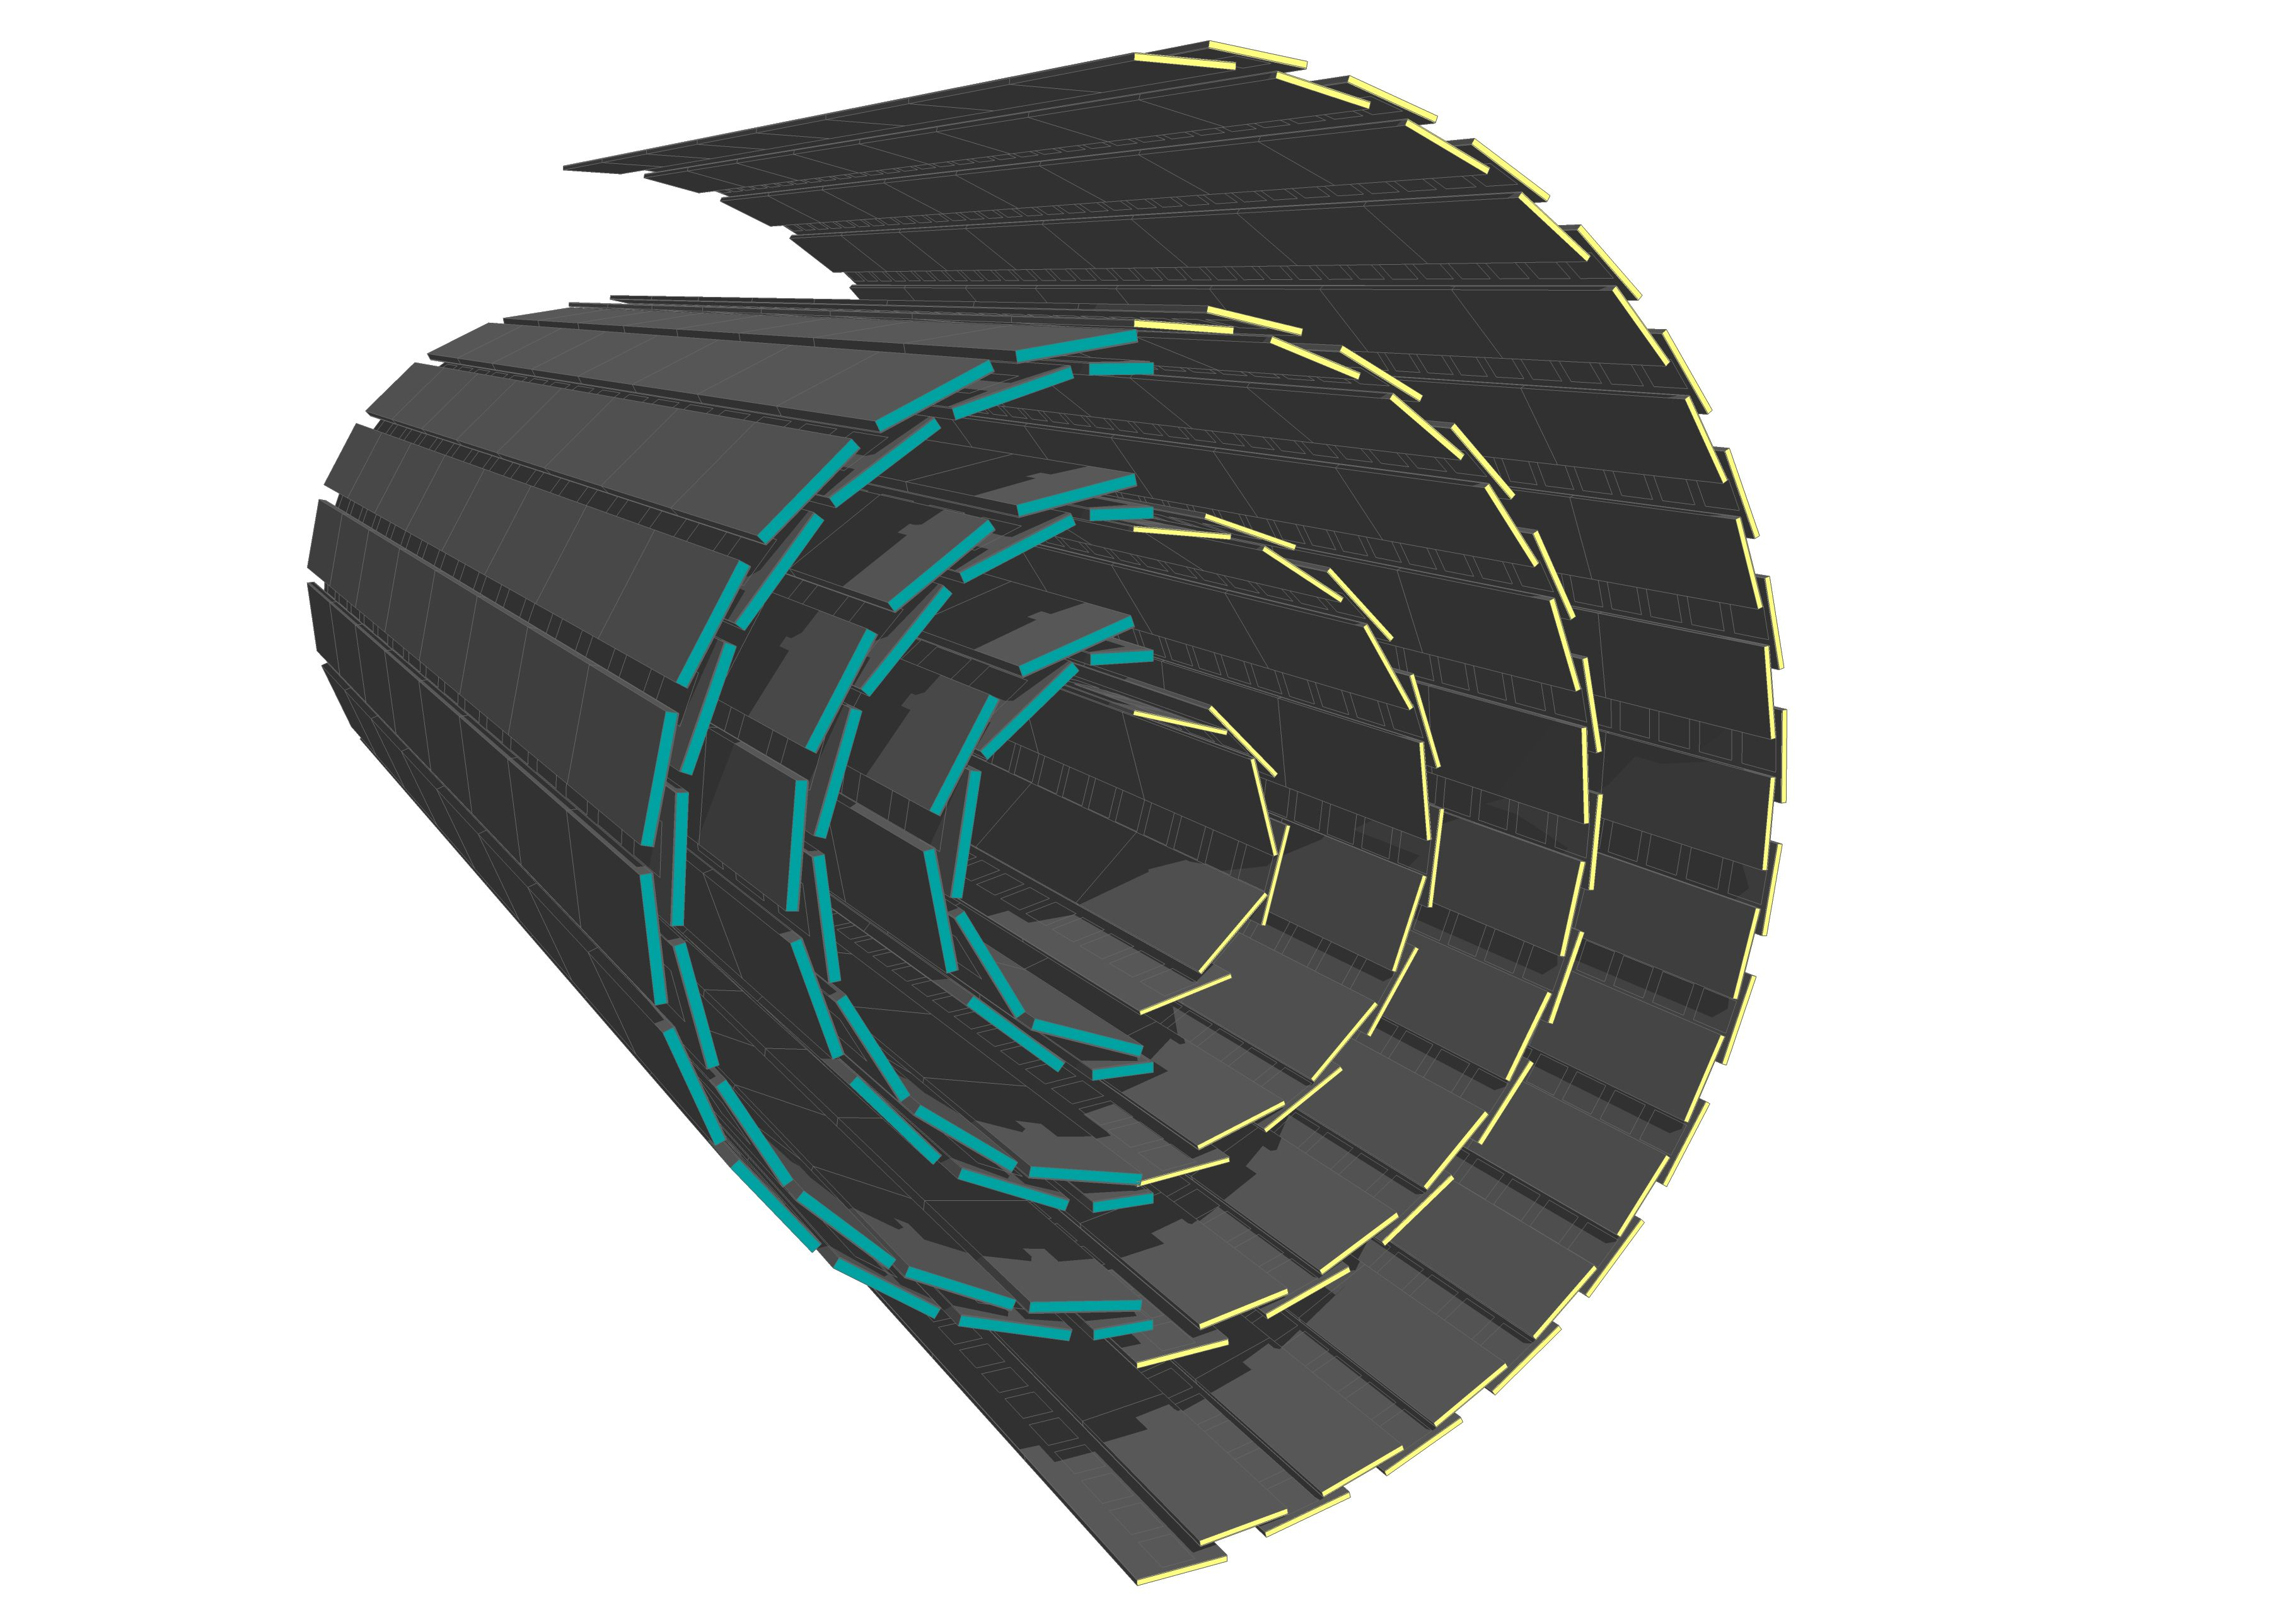
\includegraphics[width=1.0\textwidth]{021_pixel_upgrade/plots/pixel_phase1_4_layers.png}
 \caption{The model of the barrel pixel tracker before (on the left) and after the Phase 1 upgrade (on the right).}
 \label{fig:tracker_4}
\end{figure}

Addition of the fourth layer increases the amount of material which the particles have to go through. This is not
the desired feature for the innermost detectors. There are several ways planned to decrease the material amount on the 
way of the particle. So the volume of the material, which the detector is made of, has to be decreased. 
First of all, the readout system itself is planned to be thinner (it is easy to see in the Fig. \ref{fig:tracker_4},
where the new pixel barrels are thinner). And secondly, the cooling system will be changed to the $CO_{2}$ cooling \cite{CMS:2012sda} with 
light-weight mechanical support, allowing the electronic boards to be moved out of the detector volume.

The improvements planned will lead to the higher efficiencies, lower fake track rates (see sec. \ref{ssec:trkReco}), lower read-out dead time,
and extended lifetime of the detector. This results the better identification of the particles for offline analysis and HLT.

The planned upgraded detector performance was simulated. It was compared to the performance of the non-upgraded tracker. This comparison
is shown in Fig. \ref{fig:sim_perform}. These simulations were performed on the $t\bar{t}$ samples. The studies show overall higher 
efficiencies and lower fake rates for the higher pule-up scenarios.

\begin{figure}[t]
 \centering
 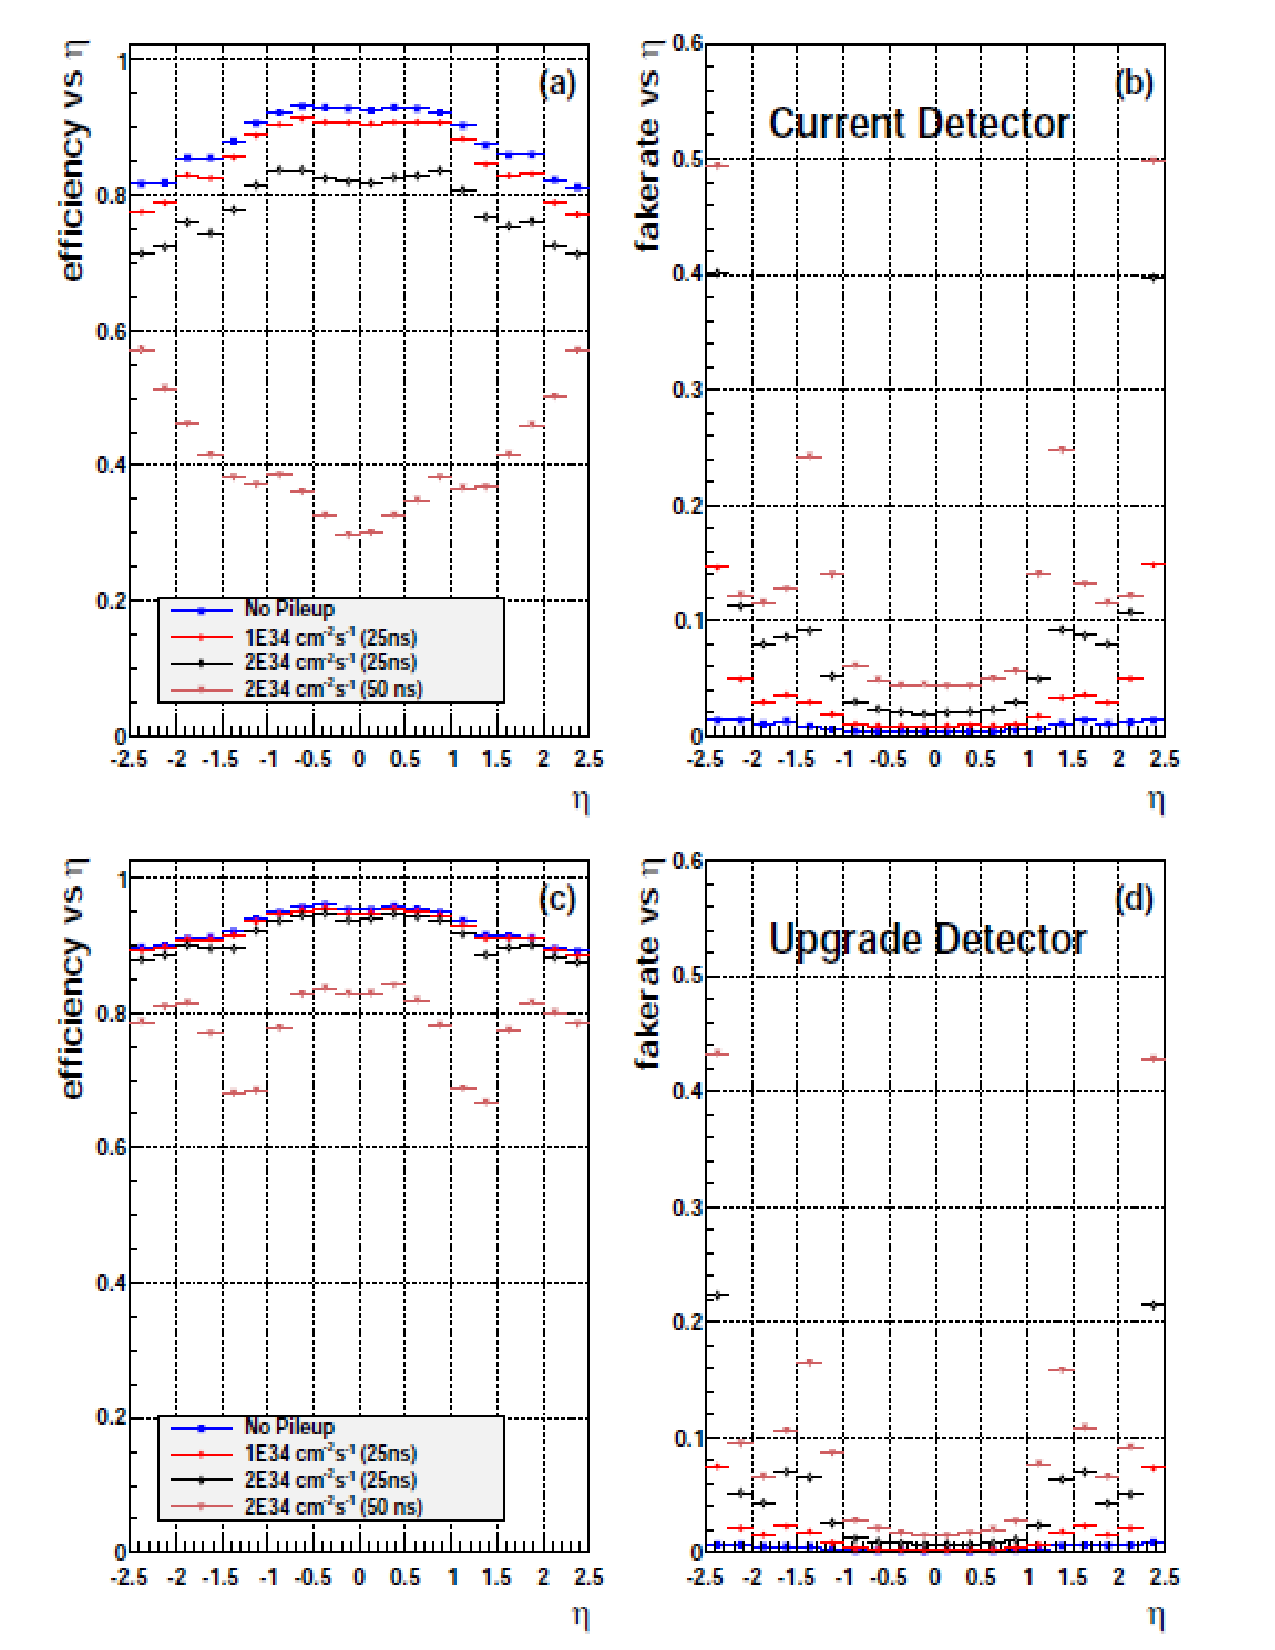
\includegraphics[width=0.8\textwidth]{021_pixel_upgrade/plots/sim_perform.pdf}
 \caption{Tracking efficiency (a,c) and fake rate (b,d) for the $t\bar{t}$ sample as a function of track
          pseudorapidity $\eta$, for the current detector (a,b) and the upgrade pixel detector (c,d). Results are shown for
          zero pileup (blue squares), an average pileup of 25 (red dots), an average pileup of 50 (black
          diamonds), and an average pileup of 100 (brown triangles) with ROC data loss simulation
          expected at the given luminosities. The plot is taken from \cite{CMS:2012sda}.}
 \label{fig:sim_perform}
\end{figure}

